\label{sec:2.1}

%%%%%%%%%%%%%%%%
% (LIN) CTS
%%%%%%%%%%%%%%%%

One of the cryogenic equipments used in ColdADC testing is the Cryogenic Test System (CTS), shown in Figure~\ref{fig:cts}. The CTS is a cryogenic test chamber mounted on top of a commerical LN$_2$ dewar. The device-under-test (e.g. ColdADC chip) can be mounted inside the test chamber and immersed in LN$_2$. The CTS can also circulate either cold or warm gas to slowly cool down or warm up the ASIC before and after testing. The CTS has been effective at minimizing water condensation on the ASIC from thermal cycling. Multiple CTS units were built by a group from Michigan State University and distributed to the various testing sites.
\begin{figure}[htb]
\centering
%\begin{minipage}[b]{1.0\textwidth}
\begin{center}
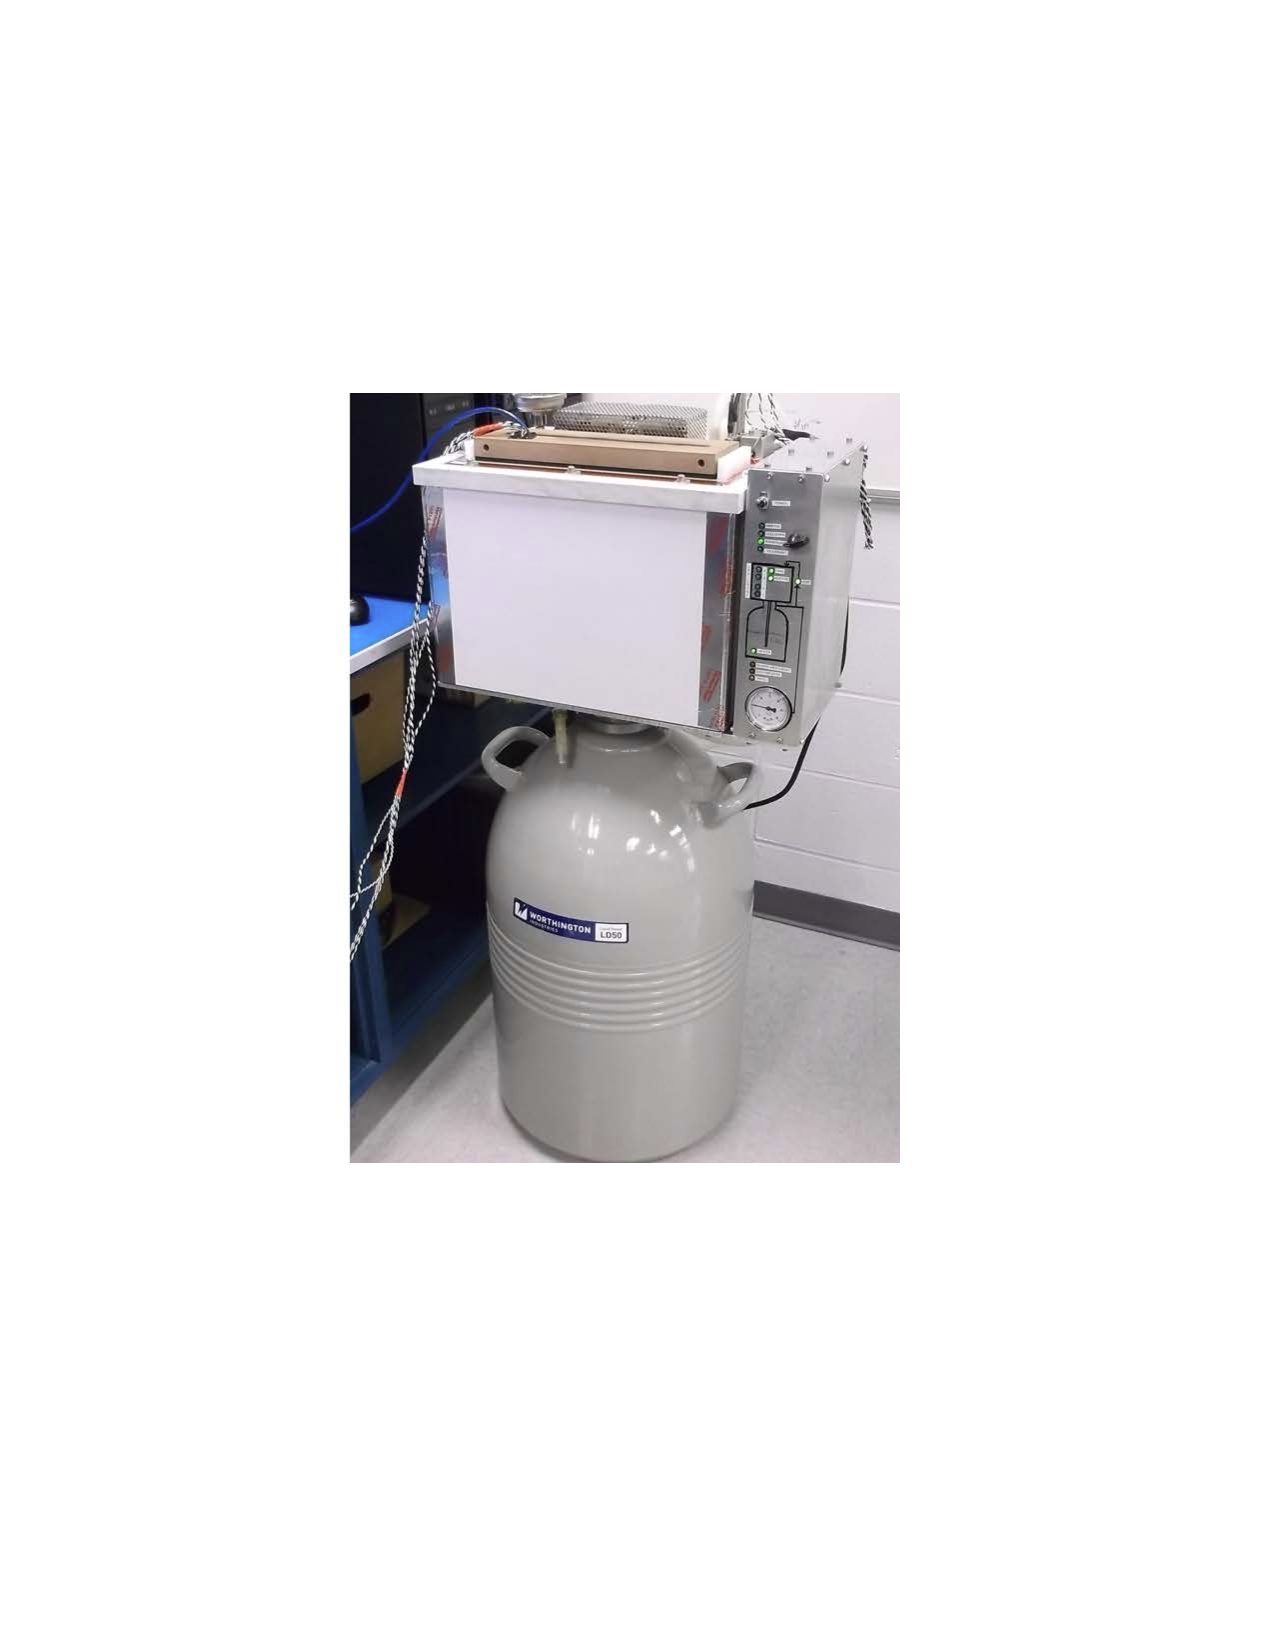
\includegraphics[width=0.5\textwidth]{figures/CTS.pdf}
\end{center}
%\end{minipage}
\caption{Cryogenic Test System.}
\label{fig:cts}
\end{figure}

